\documentclass[a4paper,12pt]{report}
\usepackage{amssymb}

\usepackage{ucs}
\usepackage[utf8x]{inputenc} % Input encoding for Greek characters
\usepackage[greek,english]{babel} % Language support

\newcommand{\en}{\selectlanguage{english}}
\newcommand{\gr}{\selectlanguage{greek}}

% \usepackage{algorithm2e}
% \usepackage{algorithm}
% \usepackage{algorithmic}
\usepackage{enumitem}
\usepackage{tcolorbox}
\tcbuselibrary{listingsutf8}
\usepackage{float}
\usepackage{amsmath}
\usepackage{graphicx} % For including images
\usepackage{titlesec} % Custom title formatting
\usepackage{fancyhdr} % For custom headers and footers
\usepackage{geometry} % For adjusting page margins

% Adjust the page margins to make content wider
\geometry{top=2.5cm, bottom=2.5cm, left=2.5cm, right=2.5cm}

% Redefine chapter formatting to make it smaller
\titleformat{\chapter}[display]
    {\normalfont\LARGE\bfseries} % Smaller size and bold for chapter heading
    {\chaptername\ \thechapter} % Chapter number format
    {15pt} % Space between chapter number and title
    {\bfseries} % Smaller size and bold for chapter title
\begin{document}

\begin{titlepage}
    \centering
    \vspace*{-3cm}
    % University logo
    \includegraphics[width=1\textwidth]{auth_logo.png} % Replace with your actual logo file

    % University name in Greek
    \textbf{\gr ΑΡΙΣΤΟΤΕΛΕΙΟ ΠΑΝΕΠΙΣΤΗΜΙΟ ΘΕΣΣΑΛΟΝΙΚΗΣ}
    \vspace{2cm}

    % Document title and subtitle in Greek
    \LARGE\textbf{\gr Γραφική με Υπολογιστές Αναφορά} \\
    \Large\normalfont{\gr Εργασία 3} \\
    \vspace{4cm}

    \gr
    \large
    \textbf{Διακολουκάς Δημήτριος} \\
    \textbf{AEM 10642}
    \vspace{2.5cm}

    \en
    \textit{Email: ddiakolou@ece.auth.gr}
\end{titlepage}

\gr
\tableofcontents

\chapter{Περιγραφή Προβλήματος και Ζητούμενα}

\section{Εισαγωγή}

Η τρίτη εργασία της σειράς μαθημάτων \textit{Γραφική με Υπολογιστές} εστιάζει στη δημιουργία ενός πλήρους \en rendering pipeline \gr για την απεικόνιση \en 3D \gr αντικειμένων υπό φωτισμό. Το σύστημα αυτό βασίζεται στη γεωμετρική και φυσική μοντελοποίηση φωτός και υλικών, αξιοποιώντας τις υλοποιήσεις των προηγούμενων εργασιών (\en transformations, projection, rasterization\gr) και επεκτείνοντάς τες με υποστήριξη φωτισμού τύπου \en Phong \gr και σκιασμού \en Gouraud \gr και \en Phong\gr.

\vspace{0.3cm}

\hspace{-0.6cm}Καλούμαστε να υλοποιήσουμε απεικόνιση ενός δεδομένου \en 3D \gr αντικειμένου, αξιοποιώντας μία εικόνα υφής και δεδομένα καμπύλωσης επιφάνειας (κανονικά διανύσματα), ώστε να παραχθούν στατικά \en frames \gr  (εικόνες) υπό διαφορετικές παραμέτρους φωτισμού και σκιασμού σύμφωνα με μεθόδους που ενδείκνυνται στην εκφώνηση.

\vspace{0.3cm}

\section{Δοσμένα Δεδομένα – \en \texttt{hw3.npy} \gr και δοθείσα εικόνα}

Το αρχείο \en \texttt{hw3.npy} \gr περιέχει όλα τα δεδομένα της σκηνής που απαιτούνται για την παραγωγή εικόνων υπό φωτισμό. Επίσης για την υλοποίηση της εργασίας δόθηκε και μία εικόνα με αναπαράσταση της \en \textbf{\textit{Mona Lisa}} \gr ονόματι \en \textit{Mona-Lisa-Exist-in-Real-Life-2635825581.png}\gr. Τα δεδομένα είναι:

\begin{itemize}
    \item \en \textbf{v\_pos:} \gr $3 \times N$ πίνακας με τις συντεταγμένες των κορυφών του αντικειμένου.
    \item \en \textbf{v\_uvs:} \gr $N \times 2$ πίνακας με τις \en UV \gr συντεταγμένες υφής για κάθε κορυφή.
    \item \en \textbf{t\_pos\_idx:} \gr $F \times 3$ πίνακας που ορίζει τα τρίγωνα μέσω δεικτών στις κορυφές.
    \item \en \textbf{tex:} \gr Εικόνα υφής του αντικειμένου.
    \item \en \textbf{cam\_pos, target, up:} \gr Συντεταγμένες κάμερας και προσανατολισμού της.
    \item \en \textbf{plane\_w, plane\_h, focal, res\_w, res\_h:} \gr Γεωμετρικά χαρακτηριστικά και ανάλυση του \en image plane\gr.
    \item \en \textbf{l\_pos:} \gr Θέσεις σημειακών πηγών φωτός (\en point lights\gr).
    \item \en \textbf{l\_int:} \gr Εντάσεις των πηγών φωτός (\en light intensity\gr).
    \item \en \textbf{l\_amb:} \gr Ένταση περιβαλλοντικού φωτισμού (\en ambient light\gr).
    \item \en \textbf{ka, kd, ks, n:} \gr Συντελεστές υλικού \en (ambient, diffuse, specular, Phong exponent)\gr.
\end{itemize}

\hspace{-0.6cm}Η εικόνα που δόθηκε για την υλοποίηση της εργασίας είναι η παρακάτω:

\begin{figure}[H]
    \centering
    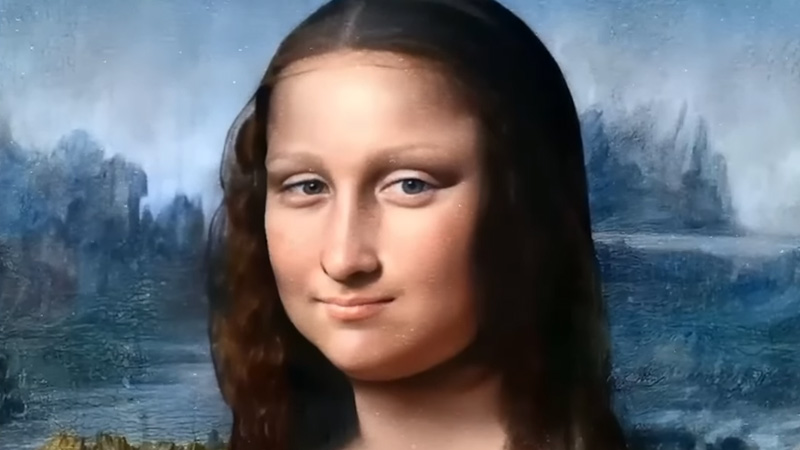
\includegraphics[width=0.7\textwidth]{Mona-Lisa-Exist-in-Real-Life-2635825581.jpg}
    \caption{\en Reference \gr εικόνα υφής από τα δεδομένα.}
    \label{fig:Mona_Lisa}
\end{figure}

\vspace{0.3cm}

\section{Ζητούμενα}

Η εργασία απαιτεί την υλοποίηση συστήματος φωτισμού και σκιασμού. Πιο αναλυτικά:

\begin{enumerate}
    \item \en \textbf{MatPhong:} \gr Κλάση που περιγράφει τα χαρακτηριστικά του υλικού ενός αντικειμένου.
    \item \en \textbf{light(...):} \gr Συνάρτηση υπολογισμού της έντασης φωτός σε σημείο επιφάνειας υπό το μοντέλο \en Phong\gr.
    \item \en \textbf{calc\_normals(...):} \gr Υπολογισμός \en normals \gr διανυσμάτων επιφάνειας για κάθε κορυφή του πλέγματος.
    \item \en \textbf{render\_object(...):} \gr Κεντρική συνάρτηση που καλεί τις υπόλοιπες και αποδίδει μία πλήρη εικόνα της σκηνής.
    \item \en \textbf{shade\_gouraud(...):} \gr Υλοποιεί σκιασμό \en Gouraud \gr σε τρίγωνα.
    \item \en \textbf{shade\_phong(...):} \gr Υλοποιεί σκιασμό \en Phong \gr με παρεμβολή στα διανύσματα και στις \en UV \gr συντεταγμένες.
\end{enumerate}

\newpage 

\section{Προσομοιώσεις και Απαιτήσεις}

Η εργασία απαιτεί την παραγωγή $8$ εικόνων:

\begin{enumerate}
    \item Τέσσερις εικόνες με χρήση σκιασμού \en Gouraud\gr:
    \begin{itemize}
        \item μόνο \en ambient \gr φωτισμός,
        \item μόνο \en diffuse \gr φωτισμός,
        \item μόνο \en specular \gr φωτισμός,
        \item συνδυασμός και των τριών.
    \end{itemize}
    \item Τέσσερις αντίστοιχες εικόνες με χρήση σκιασμού \en Phong\gr.
\end{enumerate}

\hspace{-0.6cm}Επιπλέον, ζητείται να παραχθούν εικόνες με:

\begin{itemize}
    \item Κάθε σημειακή πηγή φωτός ξεχωριστά.
    \item Όλες οι πηγές μαζί \en (combined lighting)\gr.
\end{itemize}

\hspace{-0.6cm}Όλες οι εικόνες θα αποθηκευτούν από το αρχείο \en \texttt{demo.py}\gr, το οποίο πρέπει να τρέχει χωρίς εξωτερικά ορίσματα.

\chapter{Περιληπτική περιγραφή βοηθητικών συναρτήσεων}

\section{Συνάρτηση γραμμικής παρεμβολής μεταξύ διανυσμάτων}

Η \en \texttt{vector\_interp(p1, p2, V1, V2, coord, dim)} \gr υλοποιεί γραμμική παρεμβολή μεταξύ δύο διανυσμάτων $V_1$, $V_2$ που αντιστοιχούν σε δύο σημεία $p_1$ και $p_2$:

\begin{itemize}
    \item Αν $p_1[\texttt{\en dim\gr}] = p_2[\texttt{\en dim\gr}]$, επιστρέφεται το $V_1$.
    \item Αλλιώς, υπολογίζεται συντελεστής $t = \frac{coord - p_1}{p_2 - p_1}$ και επιστρέφεται το παρεμβολημένο διάνυσμα $V = (1 - t) \cdot V_1 + t \cdot V_2$.
\end{itemize}

\hspace{-0.6cm}Χρησιμοποιείται εκτενώς σε \en scanline rendering \gr για την εύρεση τιμών εντός τριγώνου.

\vspace{0.3cm}

\section{Συστήματα Συντεταγμένων και Προβολές}

Παρακάτω περιγράφοται οι συναρτήσεις που χρησιμοποιήθηκαν και σε προηγούμενη εργασία για επεξεργασία σε συστήματα συντεταγμένων και προβολές. Πιο συγκεκριμένα:

\begin{itemize}
    \item \en \texttt{world2view(pts, R, c0)}\gr: Μετασχηματίζει σημεία από τον παγκόσμιο χώρο στο σύστημα συντεταγμένων της κάμερας με χρήση περιστροφής $R$ και θέσης κάμερας $c_0$.
\begin{tcolorbox}[colback=gray!5!white, colframe=black!75!black, title=\en Pseudo-code \gr για \en \texttt{world2view}\gr]
\en
\begin{verbatim}
function world2view(pts, R, c0):
    if pts not 3xN:
        pts = transpose(pts)
    pts_cam = R @ (pts - c0)
    return transpose(pts_cam)
\end{verbatim}
\gr
\end{tcolorbox}
    \item \en \texttt{lookat(eye, up, target)}\gr: Δημιουργεί τον πίνακα περιστροφής κάμερας ώστε να κοιτάζει από το σημείο \en \texttt{eye} \gr προς το \en \texttt{target}\gr, με προσανατολισμό το διάνυσμα \en \texttt{up}\gr. Επιστρέφει τον πίνακα περιστροφής $R$ και τη θέση κάμερας.
\begin{tcolorbox}[colback=gray!5!white, colframe=black!75!black, title=\en Pseudo-code \gr για \en \texttt{lookat}\gr]
\en
\begin{verbatim}
function lookat(eye, up, target):
    z = normalize(target - eye)
    x = normalize(cross(z, up))
    y = cross(x, z)
    R = [x, y, -z] as columns
    return R, eye
\end{verbatim}
\gr
\end{tcolorbox}
    \item \en \texttt{perspective\_project(pts, focal, R, t)}\gr: Πραγματοποιεί προβολή προοπτικής σημείων βάσει εστιακής απόστασης \en \texttt{focal} \gr και της θέσης/προσανατολισμού κάμερας. Επιστρέφει τις \en 2D \gr προβολές και τις αποστάσεις βάθους.
\begin{tcolorbox}[colback=gray!5!white, colframe=black!75!black, title=\en Pseudo-code \gr για \en \texttt{perspective\_project}\gr]
\en
\begin{verbatim}
function perspective_project(pts, focal, R, t):
    pts_cam = world2view(pts, R, t)
    for each pt in pts_cam:
        x' = focal * pt[0] / pt[2]
        y' = focal * pt[1] / pt[2]
    return [x', y'], depths
\end{verbatim}
\gr
\end{tcolorbox}
\end{itemize}

\hspace{-0.6cm}Οι παραπάνω συναρτήσεις αποτελούν θεμελιώδη συστατικά ενός \en rendering pipeline\gr, καθώς καθορίζουν τη μετάβαση από την περιγραφή της σκηνής στον παγκόσμιο χώρο (\en world coordinate system\gr) στο σύστημα της κάμερας και τελικά στην προβολή επί του επιπέδου εικόνας. Η ορθότητα και η συνέπεια στους μετασχηματισμούς αυτούς είναι κρίσιμη για τη ρεαλιστική απεικόνιση της σκηνής υπό προοπτική.

\vspace{0.3cm}

\section{Συσχέτιση με Επίπεδο Εικόνας}

Παρακάτω περιγράφεται η συνάρτηση για μετατροπή σε εικονοστοιχεία που χρησιμοποιήθηκε και υλοποιήθηκε και στην Εργασία 2. Πιο συγκεκριμένα, η συνάρτηση \en \texttt{rasterize(pts\_2d, plane\_w, plane\_h, res\_w, res\_h)} \gr μετατρέπει τις συντεταγμένες από το επίπεδο της κάμερας (\en camera plane\gr) σε συντεταγμένες εικονοστοιχείων (\en pixel coordinates\gr), λαμβάνοντας υπόψη την ανάλυση και τις φυσικές διαστάσεις του αισθητήρα προβολής. Η συνάρτηση αυτή εξασφαλίζει ότι η απεικόνιση του αντικειμένου προβάλλεται σωστά πάνω στο \en image plane \gr του τελικού \en render\gr.

\begin{tcolorbox}[colback=gray!5!white, colframe=black!75!black, title=\en Pseudo-code \gr για \en \texttt{rasterize}\gr]
\en
\begin{verbatim}
function rasterize(pts_2d, plane_w, plane_h, res_w, res_h):
    scale_x = res_w / plane_w
    scale_y = res_h / plane_h
    center_x = res_w / 2
    center_y = res_h / 2
    for each (x, y) in pts_2d:
        px = round(x * scale_x + center_x)
        py = round(-y * scale_y + center_y)
        px, py = clamp(px, py)
    return [px, py]
\end{verbatim}
\gr
\end{tcolorbox}

\vspace{0.3cm}

\hspace{-0.6cm}Όλες οι παραπάνω συναρτήσεις είναι απαραίτητες για τη δημιουργία ενός πλήρους \en pipeline \gr απόδοσης που ξεκινά από γεωμετρική αναπαράσταση και καταλήγει σε τελική εικόνα.

\vspace{0.2cm}

\hspace{-0.6cm}Η υλοποίηση των συναρτήσεων που περιέγραψα έχουν υλοποιηθεί στο αρχείο \en all\_funcs\_prev.py\gr.

\chapter{Μοντελοποίηση Φωτισμού και Υλικού Επιφάνειας}

\section{Θεωρητικό Υπόβαθρο}

Η παρούσα ενότητα περιγράφει την υλοποίηση φωτισμού επιφανειών βάσει του κλασικού μοντέλου \en Phong reflection model\gr. Το μοντέλο αυτό αποτελεί μία εμπειρική προσέγγιση της αλληλεπίδρασης φωτός και υλικού, με στόχο τη δημιουργία ρεαλιστικής απόδοσης φωτεινότητας ανά σημείο στην επιφάνεια ενός αντικειμένου.

\vspace{0.2cm}

\hspace{-0.6cm}Ο συνολικός φωτισμός σε ένα σημείο αποτελείται από τρεις επιμέρους συνιστώσες:

\begin{itemize}
    \item \textbf{\en Ambient\gr:} Aναπαριστά το φως που φτάνει έμμεσα στο σημείο λόγω ανάκλασης από άλλες επιφάνειες.
    
    \item \textbf{\en Diffuse\gr:} Προκύπτει από την ευθεία πρόσκρουση του φωτός στο σημείο, εξαρτάται από τη γωνία του φωτισμού ως προς το κάθετο διάνυσμα της επιφάνειας.
    
    \item \textbf{\en Specular\gr:} Μοντελοποιεί τη γυαλάδα και είναι ισχυρότερη όσο περισσότερο συμπίπτει η κατεύθυνση του παρατηρητή με την κατεύθυνση ανάκλασης.
\end{itemize}

\vspace{0.3cm}

\section{Κλάση \en \texttt{MatPhong}\gr}

Για να περιγραφούν τα χαρακτηριστικά του υλικού κάθε επιφάνειας, ορίζεται η κλάση \en \texttt{MatPhong}\gr. Κάθε υλικό προσδιορίζεται από τέσσερις παραμέτρους:

\begin{itemize}
    \item \en \texttt{ka} \gr: Συντελεστής \en ambient \gr συνιστώσας.
    \item \en \texttt{kd} \gr: Συντελεστής \en diffuse \gr συνιστώσας.
    \item \en \texttt{ks} \gr: Συντελεστής \en specular \gr συνιστώσας.
    \item \en \texttt{n} \gr: Εκθέτης \en Phong \gr που καθορίζει την εστίαση της λάμψης (όσο μεγαλύτερος τόσο πιο έντονο και περιορισμένο το specular).
\end{itemize}

\vspace{0.3cm}

\section{Συνάρτηση \en \texttt{light}\gr}

Η βασική συνάρτηση φωτισμού είναι η \en \texttt{light(...)} \gr και υλοποιεί το μοντέλο \en Phong \gr ανά σημείο της επιφάνειας. Η συνάρτηση δέχεται ως είσοδο τη θέση ενός σημείου της επιφάνειας, το κανονικό διάνυσμα, το χρώμα κορυφής, τη θέση της κάμερας, τις ιδιότητες του υλικού και τις παραμέτρους φωτισμού της σκηνής (φωτεινές πηγές, εντάσεις, ambient φωτισμό).

\hspace{-0.6cm}Αρχικά, το κανονικό διάνυσμα $n$ κανονικοποιείται. Υπολογίζεται η \en ambient \gr συνιστώσα ως $I_{amb} = k_a \cdot I_{env} \cdot c$, όπου $I_{env}$ η περιβαλλοντική ένταση και $c$ το τοπικό χρώμα. Έπειτα, για κάθε πηγή φωτός, η οποία μπορεί να είναι μοναδική ή μέλος λίστας, υπολογίζονται:

\begin{itemize}
    \item Το διάνυσμα φωτός $L = \texttt{\en normalize\gr}(l_i - pt)$.
    \item Το διάνυσμα παρατήρησης $V = \texttt{\en normalize\gr}(cam\_pos - pt)$.
    \item Το ανακλώμενο διάνυσμα $R = \texttt{\en normalize\gr}(2(n \cdot L)n - L)$.
\end{itemize}

\hspace{-0.6cm}Έπειτα υπολογίζονται οι δύο βασικές συνεισφορές:

\begin{itemize}
    \item \textbf{\en Diffuse:} \gr $I_{diff} = k_d \cdot \max(n \cdot L, 0)$
    \item \textbf{\en Specular:} \gr $I_{spec} = k_s \cdot \max(R \cdot V, 0)^n$
\end{itemize}

\hspace{-0.6cm}Το τελικό χρώμα προστίθεται αθροιστικά από κάθε πηγή, με βάση:

\[
I = I_{ambient} + \sum_{i} I_i \cdot \left( c \cdot I_{diff}^{(i)} + I_{spec}^{(i)} \right)
\]

\hspace{-0.6cm}Οι τιμές περιορίζονται στο διάστημα $[0, 1]$ με \en \texttt{np.clip} \gr ώστε να είναι έγκυρες τιμές \en RGB\gr.

\begin{tcolorbox}[colback=gray!5!white, colframe=black!75!black, title=\en Pseudo-code \gr για \en \texttt{light(...)}\gr]
\en
\begin{verbatim}
function light(pt, nrm, vclr, cam_pos, mat, l_pos, l_int, l_amb):
    normalize nrm
    result = mat.ka * l_amb * vclr   # Ambient

    for each light in l_pos:
        L = normalize(light - pt)    # Direction to light
        V = normalize(cam_pos - pt)  # View direction
        R = normalize(2 * dot(nrm, L) * nrm - L)  # Reflection

        diff = mat.kd * max(dot(nrm, L), 0)
        spec = mat.ks * max(dot(R, V), 0) ^ mat.n

        result += l_int * vclr * diff
        result += l_int * spec

    return clamp(result, 0, 1)
\end{verbatim}
\gr
\end{tcolorbox}

\hspace{-0.6cm}Η υλοποίηση της συνάρτησης είναι σχεδιασμένη ώστε να υποστηρίζει τόσο μοναδικές όσο και πολλαπλές φωτεινές πηγές μέσω λίστας, και να χειρίζεται ορθά περιπτώσεις μη έγκυρης γωνίας μέσω του $\max(\cdot, 0)$. Τα διανύσματα \en \texttt{L}, \texttt{V} \gr και \en \texttt{R} \gr κανονικοποιούνται ώστε οι γωνιακοί υπολογισμοί να είναι αριθμητικά σταθεροί. Το αποτέλεσμα επιστρέφει το συνολικό φωτισμό στο σημείο και χρησιμοποιείται σε συναρτήσεις όπως \en \texttt{shade\_gouraud} \gr και \en \texttt{shade\_phong}\gr.

\hspace{-0.6cm}Οπτικά, η επίδραση των επιμέρους συνιστωσών ερμηνεύεται ως εξής:

\begin{itemize}
    \item \textbf{\en Ambient:} \gr εξασφαλίζει ότι ακόμη και σκιερές περιοχές έχουν κάποιο ελάχιστο φωτισμό.
    \item \textbf{\en Diffuse:} \gr προσδίδει αίσθηση όγκου μέσω γωνίας πρόπτωσης του φωτός.
    \item \textbf{\en Specular:} \gr προσδίδει γυαλάδα και την ψευδαίσθηση στιλπνότητας.
\end{itemize}


\vspace{0.2cm}

\hspace{-0.6cm}Η συνάρτηση \en \texttt{light(...)} \gr αποτελεί το βασικό οικοδομικό στοιχείο για όλες τις ρουτίνες σκιασμού που ακολουθούν, καθώς καλείται σε κάθε σημείο (ή κορυφή) για τον υπολογισμό της τελικής φωτεινότητας.

\vspace{0.3cm}

\hspace{-0.6cm}Τα παραπάνω υλοποιούνται σε \en Python \gr με σχολιασμό στο αρχείο \en MatPhong.py\gr.

\chapter{Ανάλυση Μεθόδων Σκιασμού και \en Object Rendering\gr}

Η παρούσα ενότητα παρέχει μία αναλυτική παρουσίαση και τεκμηρίωση των βασικών συναρτήσεων που χρησιμοποιούνται για την απόδοση (\en rendering) 3D \gr μοντέλων με χρήση φωτισμού τύπου \en Phong\gr, και τις δύο βασικές τεχνικές σκιασμού: \en Gouraud \gr και \en Phong\gr.

\section{Υπολογισμός Κανονικών Διανυσμάτων: \en \texttt{calc\_normals}\gr}

Η συνάρτηση \en \texttt{calc\_normals} \gr δέχεται ένα σύνολο από σημεία \en \texttt{pts} \gr $\in \mathbb{R}^{3\times N}$ και έναν πίνακα από δείκτες τριγώνων \en \texttt{t\_pos\_idx} \gr $\in \mathbb{Z}^{3\times M}$.

\hspace{-0.6cm}Για κάθε τρίγωνο με κορυφές $\vec{v}_0, \vec{v}_1, \vec{v}_2$, υπολογίζεται το κανονικό διάνυσμα επιφάνειας μέσω του:
\[
\vec{n}_f = (\vec{v}_1 - \vec{v}_0) \times (\vec{v}_2 - \vec{v}_0)
\]

\hspace{-0.6cm}Αυτό το διάνυσμα προστίθεται στις τρεις αντίστοιχες κορυφές. Τελικά, όλα τα διανύσματα κανονικοποιούνται ώστε να έχουν μοναδιαίο μέτρο.

\begin{tcolorbox}[colback=gray!5!white, colframe=black!75!black, title=\en Pseudo-code for \texttt{calc\_normals}\gr]
\en
\begin{verbatim}
function calc_normals(pts, t_pos_idx):
    nrm = zeros_like(pts)
    for each triangle:
        v0, v1, v2 = triangle vertices
        face_n = cross(v1 - v0, v2 - v0)
        add face_n to nrm at each vertex
    normalize all vectors
    return nrm
\end{verbatim}
\gr
\end{tcolorbox}

\hspace{-0.6cm}Έτσι, λοιπόν, υπολογίζει ομαλοποιημένα κανονικά διανύσματα για κάθε κορυφή βάσει των επιφανειακών \en normals \gr των τριγώνων.

\vspace{0.3cm}

\section{Σκιασμός ανά Κορυφή: \en \texttt{shade\_gouraud}\gr}

Η συνάρτηση \en \texttt{shade\_gouraud} \gr εφαρμόζει την τεχνική \en Gouraud shading\gr:

\begin{itemize}
\item Για κάθε κορυφή του τριγώνου, υπολογίζεται ο φωτισμός με τη συνάρτηση \en \texttt{light}\gr.
\item Παρεμβάλλονται οι τιμές χρώματος μεταξύ κορυφών σε κάθε \en scanline\gr.
\item Η υφή διαβάζεται μόνο μία φορά ανά κορυφή.
\end{itemize}

\begin{tcolorbox}[colback=gray!5!white, colframe=black!75!black, title=\en Pseudo-code for \texttt{shade\_gouraud}\gr]
\en
\begin{verbatim}
for i = 0 to 2:
    P_cam = v_pos[:, i]
    N_i = v_nrm[:, i]
    uv_i = v_uvs[:, i]
    texel = tex[uv_i]
    color[i] = light(P_cam, N_i, texel, ...)

for each scanline:
    compute A, B positions on scanline
    interpolate color between A and B
    for each pixel x between A and B:
        img[y, x] = interpolated color
\end{verbatim}
\gr
\end{tcolorbox}

\hspace{-0.6cm}Σε αυτή την συνάρτηση δηλαδή, υπολογίζεται ο φωτισμός στις κορυφές και παρεμβάλει το χρώμα ανά \en pixel \gr για γρήγορη απόδοση με μειωμένη ακρίβεια.

\vspace{0.3cm}

\section{Σκιασμός ανά \en Pixel\gr: \en \texttt{shade\_phong}\gr}

Η συνάρτηση \en \texttt{shade\_phong} \gr εφαρμόζει τον \en Phong shading \gr ανά \en pixel\gr:

\begin{itemize}
\item Παρεμβάλλονται κανονικά διανύσματα, υφές και θέσεις ανά \en pixel\gr.
\item Καλείται η \en \texttt{light(...)} \gr για κάθε \en pixel \gr ξεχωριστά.
\item Δίνει ομαλό και ρεαλιστικό φωτισμό ακόμη και σε \en curved \gr επιφάνειες.
\end{itemize}

\begin{tcolorbox}[colback=gray!5!white, colframe=black!75!black, title=\en Pseudo-code for \gr \en \texttt{shade\_phong}\gr]
\en
\begin{verbatim}
for each scanline:
    compute A, B screen positions
    interpolate normals, UVs, and 3D positions from A to B
    for each pixel x between A and B:
        texel = tex[UV]
        color = light(P, N, texel, ...)
        img[y, x] = color
\end{verbatim}
\gr
\end{tcolorbox}

\hspace{-0.6cm}Η συνάρτηση αυτή συνοπτικά υπολογίζει φωτισμό για κάθε \en pixel\gr, επιτυγχάνοντας πολύ ρεαλιστική απόδοση με υψηλό υπολογιστικό κόστος.

\vspace{0.3cm}

\section{Απόδοση Αντικειμένου: \en \texttt{render\_object}\gr}

Η συνάρτηση \en \texttt{render\_object} \gr είναι η βασική ρουτίνα απόδοσης (\en rendering pipeline\gr) και εκτελεί τα εξής:

\begin{enumerate}
\item Υπολογίζει κανονικά μέσω \en \texttt{calc\_normals}\gr.
\item Υπολογίζει μετασχηματισμούς κάμερας μέσω \en \texttt{lookat} \gr και μετασχηματίζει τις κορυφές στο χώρο της κάμερας.
\item Υλοποιεί προοπτική προβολή μέσω \en \texttt{perspective\_project}\gr.
\item Μετατρέπει συντεταγμένες σε \en pixels \gr με \en \texttt{rasterize}\gr.
\item Υπολογίζει το βάθος κάθε τριγώνου και τα σχεδιάζει με σειρά από το πίσω προς το μπροστά (\en depth sorting\gr).
\item Καλεί τη συνάρτηση σκιασμού \en \texttt{shade\_gouraud} \gr ή \en \texttt{shade\_phong} \gr ανά τρίγωνο.
\end{enumerate}

\begin{tcolorbox}[colback=gray!5!white, colframe=black!75!black, title=\en Pseudo-code for \texttt{render\_object}\gr]
\en
\begin{verbatim}
normals = calc_normals(v_pos, t_pos_idx)
R, t = lookat(eye, up, target)
v_cam = R @ v_pos + t
proj2d, depth = perspective_project(v_cam)
pix = rasterize(proj2d)
triangles = sort_by_depth(depth)

for each triangle in triangles:
    if shader == 'gouraud':
        shade_gouraud(...)
    else if shader == 'phong':
        shade_phong(...)
\end{verbatim}
\gr
\end{tcolorbox}

\hspace{-0.6cm}Η συνάρτηση αυτή πρακτικά ολοκληρώνει όλη τη ροή από υπολογισμό \en normals \gr μέχρι την τελική απόδοση του αντικειμένου στην εικόνα. 

\vspace{0.3cm}

\hspace{-0.6cm}Οι βασικές αυτές συναρτήσεις υλοποιούνται στο αρχείο \en all\_funcs\_new.py\gr.

\chapter{Κλήση Συναρτήσεων, Αποτελέσματα και Παρατηρήσεις}

Η παρούσα ενότητα περιγράφει τη διαδικασία κλήσης της συνάρτησης \en render\_object \gr μέσα από το αρχείο \en \texttt{demo.py}\gr. Ακολουθεί η απόδοση εικόνων με διαφορετικούς φωτισμούς και τεχνικές σκιασμού.

\section{Διαδικασία Εκτέλεσης}

Το πρόγραμμα:

\begin{itemize}
  \item Φορτώνει γεωμετρικά δεδομένα (θέσεις κορυφών \en v\_pos \gr, \en UVs\gr, τρίγωνα \en t\_pos\_idx\gr).
  \item Ορίζει θέση κάμερας \en eye\gr, διεύθυνση στόχευσης \en target \gr και διάνυσμα \en up \gr.
  \item Φορτώνει υφή από αρχείο ή χρησιμοποιεί λευκή υφή.
  \item Καλεί την \en render\_object \gr για κάθε συνδυασμό φωτισμού και σκιασμού.
  \item Αποθηκεύει τις εικόνες στον φάκελο \en \texttt{results/} \gr που δημιουργείται.
\end{itemize}

\section{Αποτελέσματα ανά Τεχνική Σκιασμού και Μοντέλο Φωτισμού}

Στην παρούσα ενότητα παρουσιάζονται τα αποτελέσματα απόδοσης του αντικειμένου για διαφορετικές τεχνικές σκιασμού και συνιστώσες του μοντέλου φωτισμού, με στόχο την οπτική σύγκριση και εξαγωγή συμπερασμάτων.

\begin{figure}[H]
\centering

\includegraphics[width=0.48\textwidth]{gouraud_ambient.png}
\hfill

\includegraphics[width=0.48\textwidth]{phong_ambient.png}
\caption{\en Gouraud Ambient (left) \gr και \en Phong Ambient (right)\gr}
\label{fig:gouraud_phong_ambient}
\end{figure}

\begin{figure}[H]
\centering

\includegraphics[width=0.48\textwidth]{gouraud_ambient_larger_ka.png}
\hfill
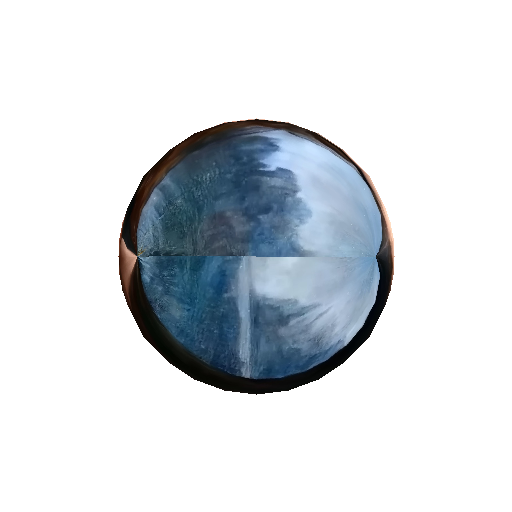
\includegraphics[width=0.48\textwidth]{phong_ambient_larger_ka.png}
\caption{\en Gouraud Ambient (ka = 1) (left) \gr και \en Phong Ambient (ka = 1) (right)\gr}
\label{fig:gouraud_phong_ambient_ka_1}
\end{figure}

\begin{figure}[H]
\centering
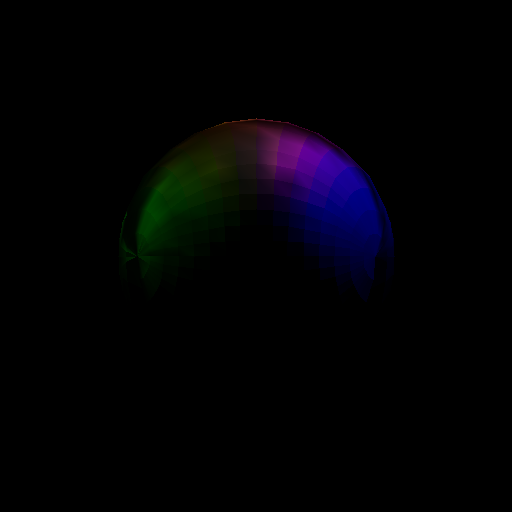
\includegraphics[width=0.48\textwidth]{gouraud_diffuse.png}
\hfill
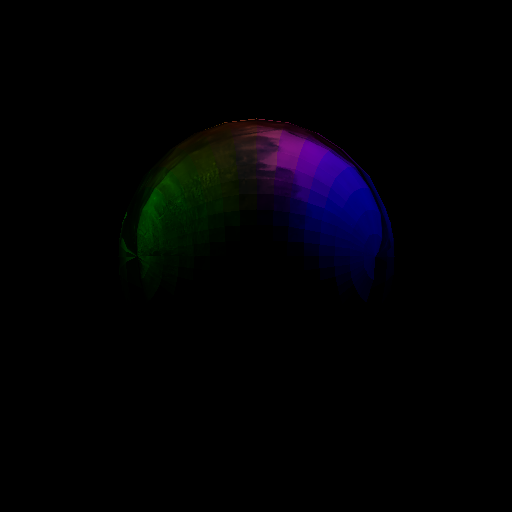
\includegraphics[width=0.48\textwidth]{phong_diffuse.png}
\caption{\en Gouraud Diffuse (left) \gr και \en Phong Diffuse (right)\gr}
\label{fig:gouraud_phong_diffuse}
\end{figure}

\begin{figure}[H]
\centering
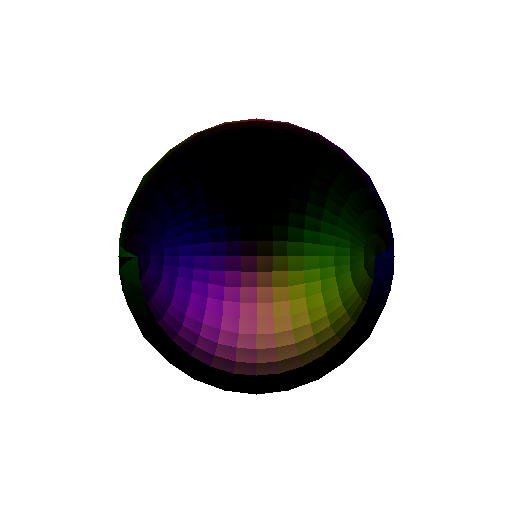
\includegraphics[width=0.48\textwidth]{gouraud_specular.png}
\hfill
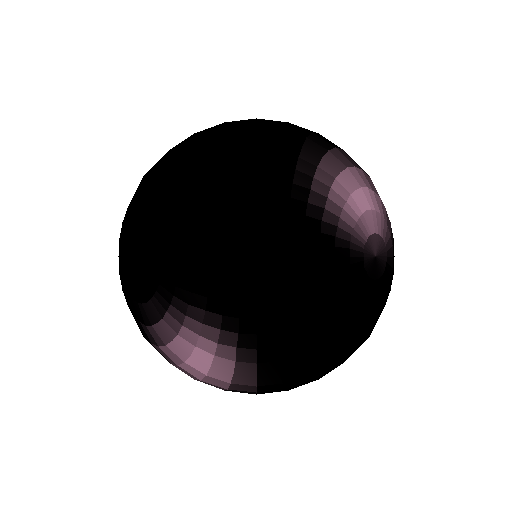
\includegraphics[width=0.48\textwidth]{phong_specular.png}
\caption{\en Gouraud Specular (left) \gr και \en Phong Specular (right)\gr}
\label{fig:gouraud_phong_specular}
\end{figure}

\begin{figure}[H]
\centering
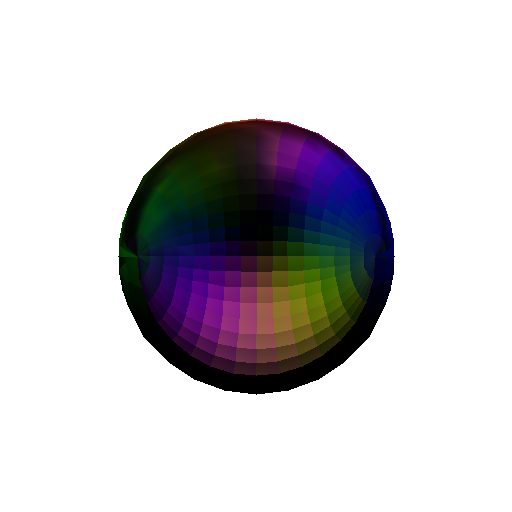
\includegraphics[width=0.48\textwidth]{gouraud_all.png}
\hfill
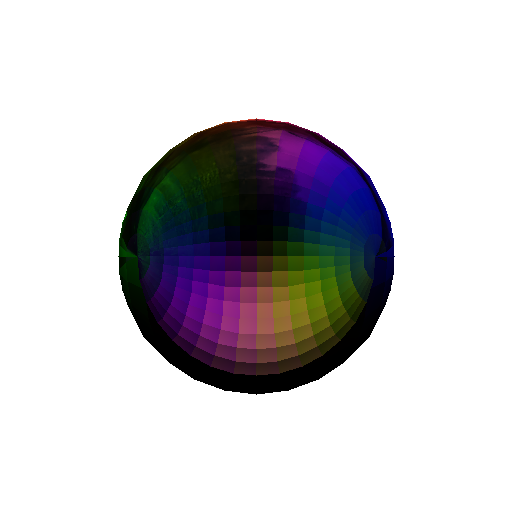
\includegraphics[width=0.48\textwidth]{phong_all.png}
\caption{\en Gouraud All (left) \gr και \en Phong All (right)\gr}
\label{fig:gouraud_phong_all}
\end{figure}

\section{Απόδοση Μεμονωμένων Πηγών Φωτός (\en Phong Only\gr)}

Σε αυτή την ενότητα εξετάζουμε την επίδραση κάθε μεμονωμένης πηγής φωτός ξεχωριστά, χρησιμοποιώντας αποκλειστικά \en Phong shading\gr, ώστε να αναδείξουμε τον ρόλο και τη συμβολή της καθεμιάς στη συνολική φωτεινότητα και εμφάνιση του αντικειμένου.

\begin{figure}[H]
\centering

\includegraphics[width=0.48\textwidth]{phong_light_1.png}
\hfill
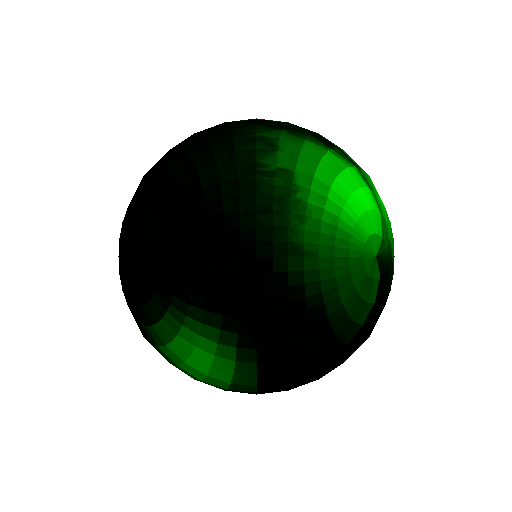
\includegraphics[width=0.48\textwidth]{phong_light_2.png}
\caption{\en Phong Light 1 (left) \gr και \en Phong Light 2 (right)\gr}
\label{fig:phong_lights_1_2}
\end{figure}

\begin{figure}[H]
\centering
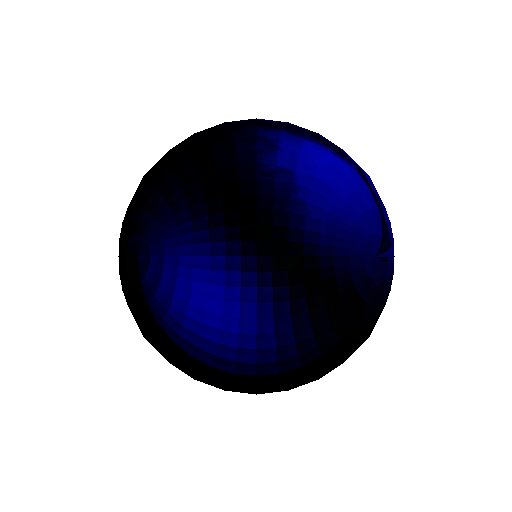
\includegraphics[width=0.48\textwidth]{phong_light_3.png}
\hfill
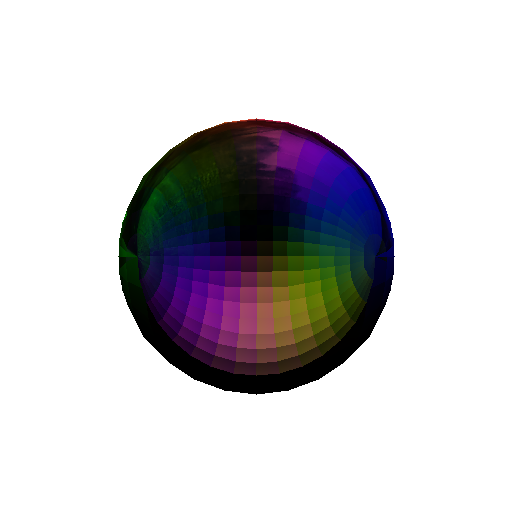
\includegraphics[width=0.48\textwidth]{phong_light_all.png}
\caption{\en Phong Light 3 (left) \gr και \en Phong All Lights (right) \gr}
\label{fig:phong_lights_3_all}
\end{figure}

\vspace{0.3cm}

\section{Συμπεράσματα και Παρατηρήσεις}

Η παρούσα εργασία ανέδειξε τη σημασία της επιλογής κατάλληλου μοντέλου σκιασμού και ρύθμισης παραμέτρων φωτισμού για ρεαλιστική απόδοση \en 3D \gr αντικειμένων.

\begin{itemize}
  \item Το \en Gouraud shading \gr είναι υπολογιστικά αποδοτικό, καθώς ο φωτισμός υπολογίζεται μόνο στις κορυφές και παρεμβάλλεται στο εσωτερικό των τριγώνων. Ωστόσο, αυτό έχει ως αποτέλεσμα την απώλεια λεπτομερειών, ειδικά στα \en specular highlights\gr, τα οποία μπορεί να «εξαφανιστούν» αν δεν βρίσκονται ακριβώς σε κορυφή. Το τελικό αποτέλεσμα ενδέχεται να φαίνεται πιο θολό ή παραμορφωμένο \en (blurred, distorted)\gr.

  \item Αντίθετα, το \en Phong shading \gr, το οποίο υπολογίζει φωτισμό ανά \en pixel\gr, προσφέρει πολύ πιο ρεαλιστική εμφάνιση, διατηρώντας λεπτομέρειες και εξομαλύνοντας τις μεταβάσεις φωτεινότητας. Η ακρίβεια στον φωτισμό είναι αισθητά βελτιωμένη, ειδικά σε καμπύλες ή λεπτομερείς επιφάνειες.

  \item Η \en ambient \gr συνιστώσα είναι υπεύθυνη για την ομοιόμορφη βασική φωτεινότητα σε ολόκληρη την επιφάνεια του αντικειμένου. Η \en diffuse \gr αντιπροσωπεύει την διάχυτη αντανάκλαση φωτός και σχετίζεται με τη γωνία πρόσπτωσης του φωτός στην επιφάνεια. Η \en specular \gr είναι υπεύθυνη για τις γυαλιστερές λάμψεις και εξαρτάται από τη γωνία ανάκλασης σε σχέση με τον παρατηρητή.

  \item Ο πλήρης φωτισμός δηλαδή ο συνδυασμός των \en ambient, diffuse \gr και \en specular \gr συνιστωσών σε συνδυασμό με την παρουσία πολλαπλών πηγών φωτός οδηγεί σε ρεαλιστικότερα και πιο αισθητικά αποτελέσματα. Ιδιαίτερα σε \en Phong shading\gr, αυτές οι πηγές φωτός αλληλεπιδρούν σωστά με την καμπυλότητα και υφή της επιφάνειας.

  \item Επιπλέον, κατά μια πειραματική εφαρμογή που εφάσμοσα, παρατηρήθηκε ότι η πολύ μικρή τιμή της παραμέτρου \en ka = 0.01 \gr (συντελεστής \en ambient \gr φωτισμού) στο αρχείο \en hw3.npy \gr είχε ως αποτέλεσμα σκοτεινές απεικονίσεις όταν χρησιμοποιούνταν μόνο \en ambient \gr φωτισμός. Αυτό αναδεικνύει τη σημασία σωστού καλιμπραρίσματος των φωτιστικών παραμέτρων ανάλογα με την υφή, το μέγεθος και την κάμερα του σκηνικού.
\end{itemize}


\hspace{-0.6cm}\textbf{Τελική Παρατήρηση:} Ο συνδυασμός \en Phong shading \gr με πλήρεις φωτιστικές συνιστώσες και πολλαπλές πηγές φωτός προσφέρει το καλύτερο δυνατό αποτέλεσμα για ρεαλιστική \en 3D \gr απόδοση. Η υπεροχή του είναι εμφανής στα διαγράμματα, όπου τα χαρακτηριστικά του αντικειμένου αποδίδονται με υψηλή πιστότητα και φυσικότητα.

\bibliographystyle{plain}
\begin{thebibliography}{1}
    \bibitem{first_bibl}
    \en https://docs.opencv.org/4.x/d9/df8/tutorial\_root.html
    \bibitem{second_bibl}
    \en https://imageio.readthedocs.io/en/stable/
\end{thebibliography}

\end{document}